% This is an example for a `Introduction'.
% To generate the final document, run latex, build and quick build commands
% on the skeleton-thesis file not this one.

\chapter{Introduction}\label{chapters:Introduction}
\vspace{-7mm}

While seemingly small objects, nuclei and their interactions can play an enormous role across a wide swath of energy and spatial scales.
From understanding the abundance of elements produced in astrophysical events to providing a general description of quantum many-body equilibration, the deceptively simple study of two colliding nuclei can be illuminating.
Even the more traditionally aligned investigations that are associated with nuclear reactions (such as superheavy element and neutron-rich nuclei formation) acts as a foundation for other areas of physics to piece together an understanding of the physical world.

Leaving aside the fact that nuclei are made of protons and neutrons, the dynamics of interacting quantum systems alone is of extreme interest to researchers from varied fields.
This is due to the striking fact that most quantum many-body systems (no matter the specific systems and particles that compose their structure) exhibit the same general features as atomic nuclei.
That is to say that studying the fusion, transfer, equilibration, vibrations, etc. of nuclear systems can provide vital insight into analogous studies in interactions between cold atoms or molecules -- systems which are several orders of magnitude larger than the few femtometers (fm) of interest to nuclear physicists.

\section{The Nuclear Many-Body Problem (in a nutshell)}

\begin{figure}
	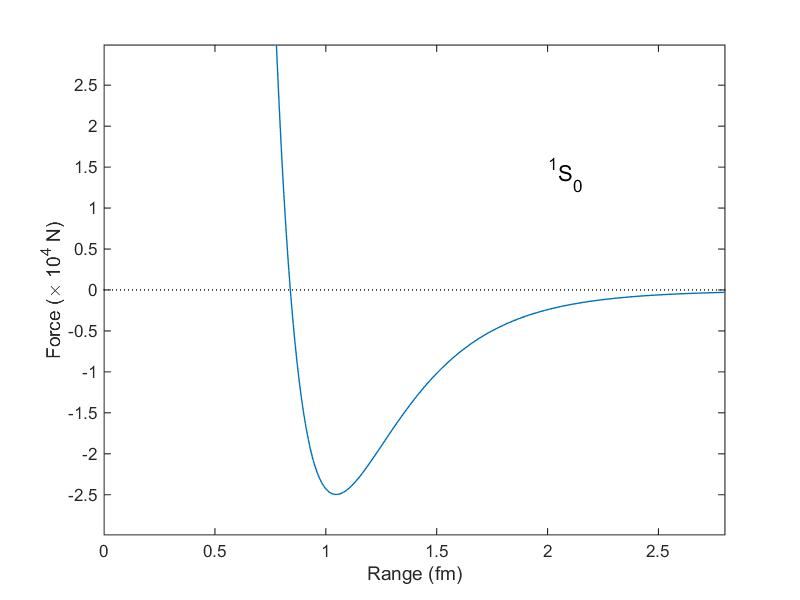
\includegraphics[width=\textwidth]{../Figures/intro_figs/ReidForce2.jpg}
	\caption{\citep{reid1968} Figure from~\citep{bdushaw}.}
\end{figure}

The specific subbranch of nuclear physics this thesis focuses on is the realm of low-energy nuclear physics.
At this level, relativistic effects are typically neglected and the nuclei are modeled as collections of protons and neutrons interacting with each other to form a bound system.
The force felt by the nucleons themselves is an artifact of the strong interaction, mediated primarily by the exchange of virtual pions with an effective range of about~$1$~(fm).
Through further contributions by vector mesons (principally rho and omega), a complicated model of interacting nucleons can be built that depends on not only a nucleon's charge and distance, but also on its spin and angular momentum as well.
Extensive effort has been placed in modeling nuclei using such an interaction (see ~\citep{wiringa1995} and~\citep{reid1968} for popular choices of a N-N potential), though this \textit{ab initio} approach is not numerically feasible for large nuclei or for dynamical interactions between nuclei.
It is for this reason that alternate approaches to modeling finite nuclei have been pursued throughout the field's history.

One such approach is that of the mean-field method \citep{hartree1928,fock1930,dirac1930,kohn1965}

The specific mean-field approaches to each project presented in this work are discussed in their respective chapters, though a general, brief word should be said about the mean-field method as it applies to atomic nuclei.
As the nucleus is traditionally thought of as a densely packed collection of nucleons, the primary assumption that individual protons and neutrons can travel freely in the nucleus is a bit counter intuitive.
It turns out, however, that the Pauli exclusion principle between nucleons ensures that the particles will remain at an average distance exceeding their radius at low energies~\citep{ring1980}.
Even at finite collision energies, the mean free path of nucleons in the nucleus is several times that of the nuclear radius, implying that a so-called hard-core collision is unlikely.
Should one go to higher energies, the mean-field approximation begins to break down and may misrepresent the outcome of such reactions.

\section{Nuclear Dynamics}

static systems rare in nature, firm understanding of dynamics and reactions

Broad picture of dynamics of nuclear systems
focus on reactions and collisions between two nuclei
Studies can be broadly separated into time scales of reactions
though in practice, experimental studies include events from all

sec1 time scales
sec2 methods to study reactions




%% Section
\section{Section 1}\label{sec:ch_1_sec_1}

%% Subsection
\subsection{Subsection 1}\label{subsec:subsec_1.1.1}


\clearpage
